\section{Diurnal temperature range}
\label{sec:DTRmonth}

In the following section, the diurnal temperature range (DTR) is investigated. The CRU TS data is analyzed by month and latitude to determine trends. 

\begin{figure}[ht]
    \centering

    \begin{subfigure}{0.48\textwidth}
        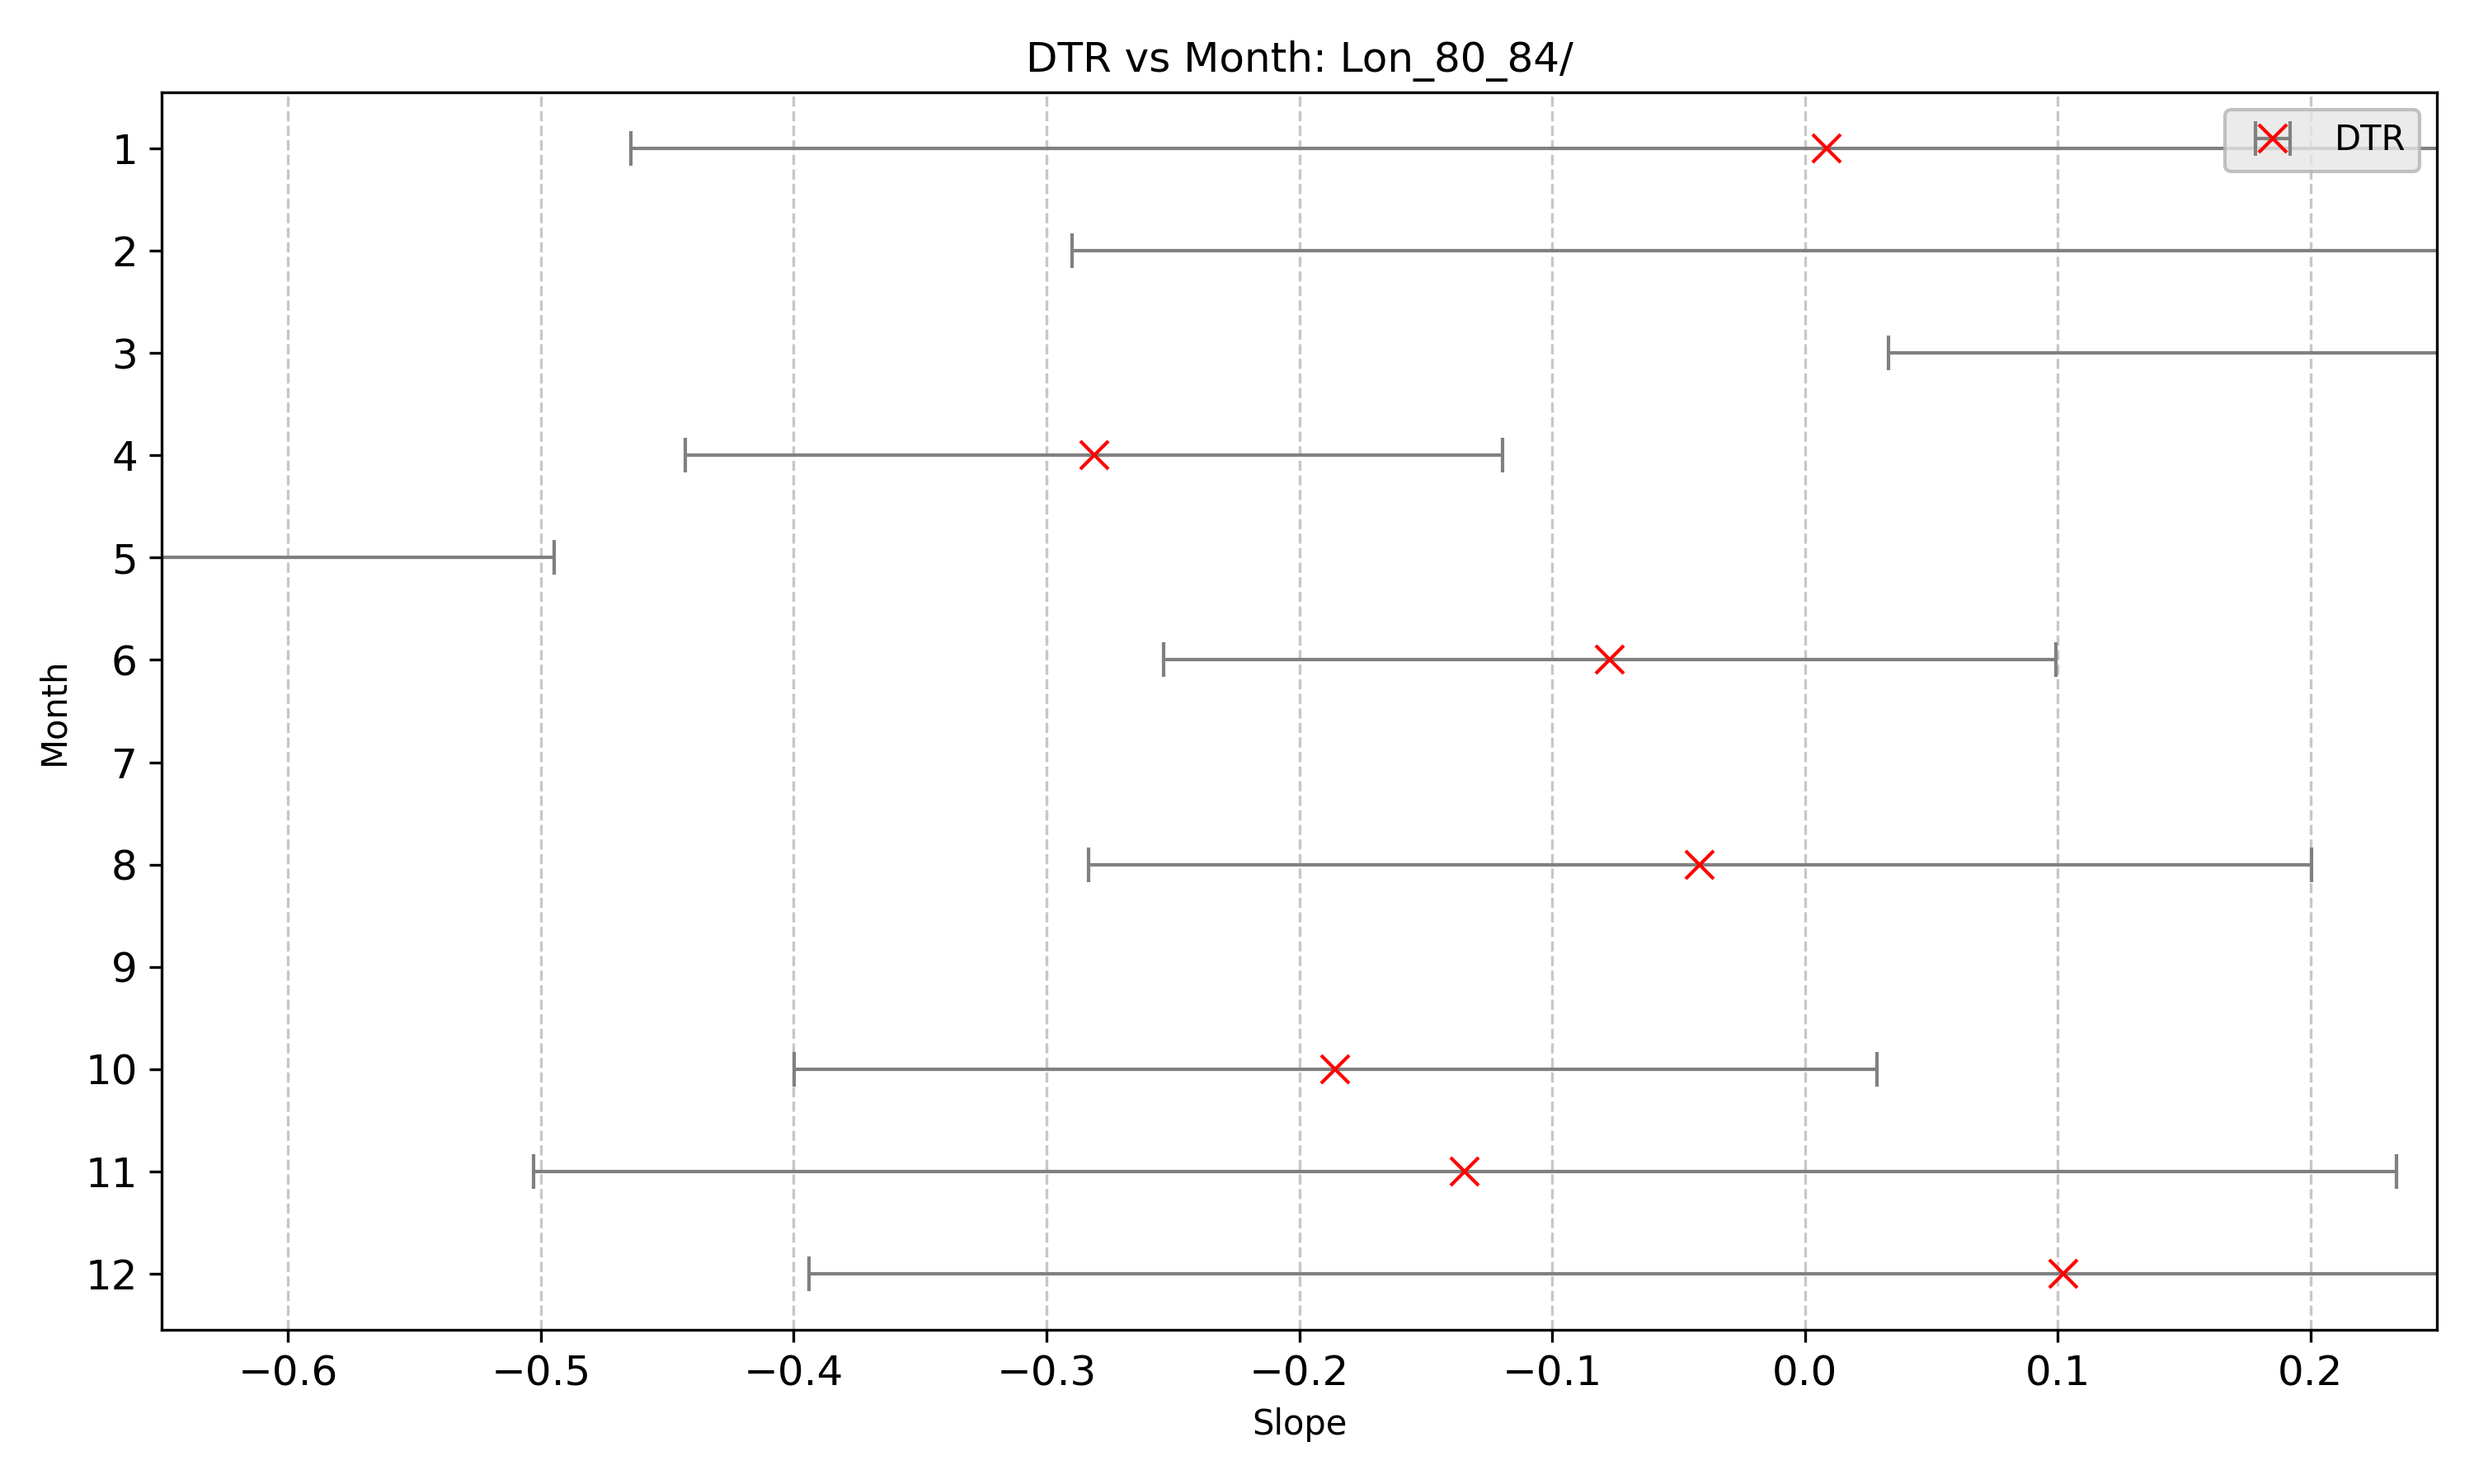
\includegraphics[width=\textwidth]{C:/Users/leonh/Desktop/Praktikum_AWI/NordPol/Lon_66_84/Fit/DTRperMonth.png}
        \caption{DTR}
        \label[type]{subfig:DTRentire}
    \end{subfigure}
    \begin{subfigure}{0.48\textwidth}
        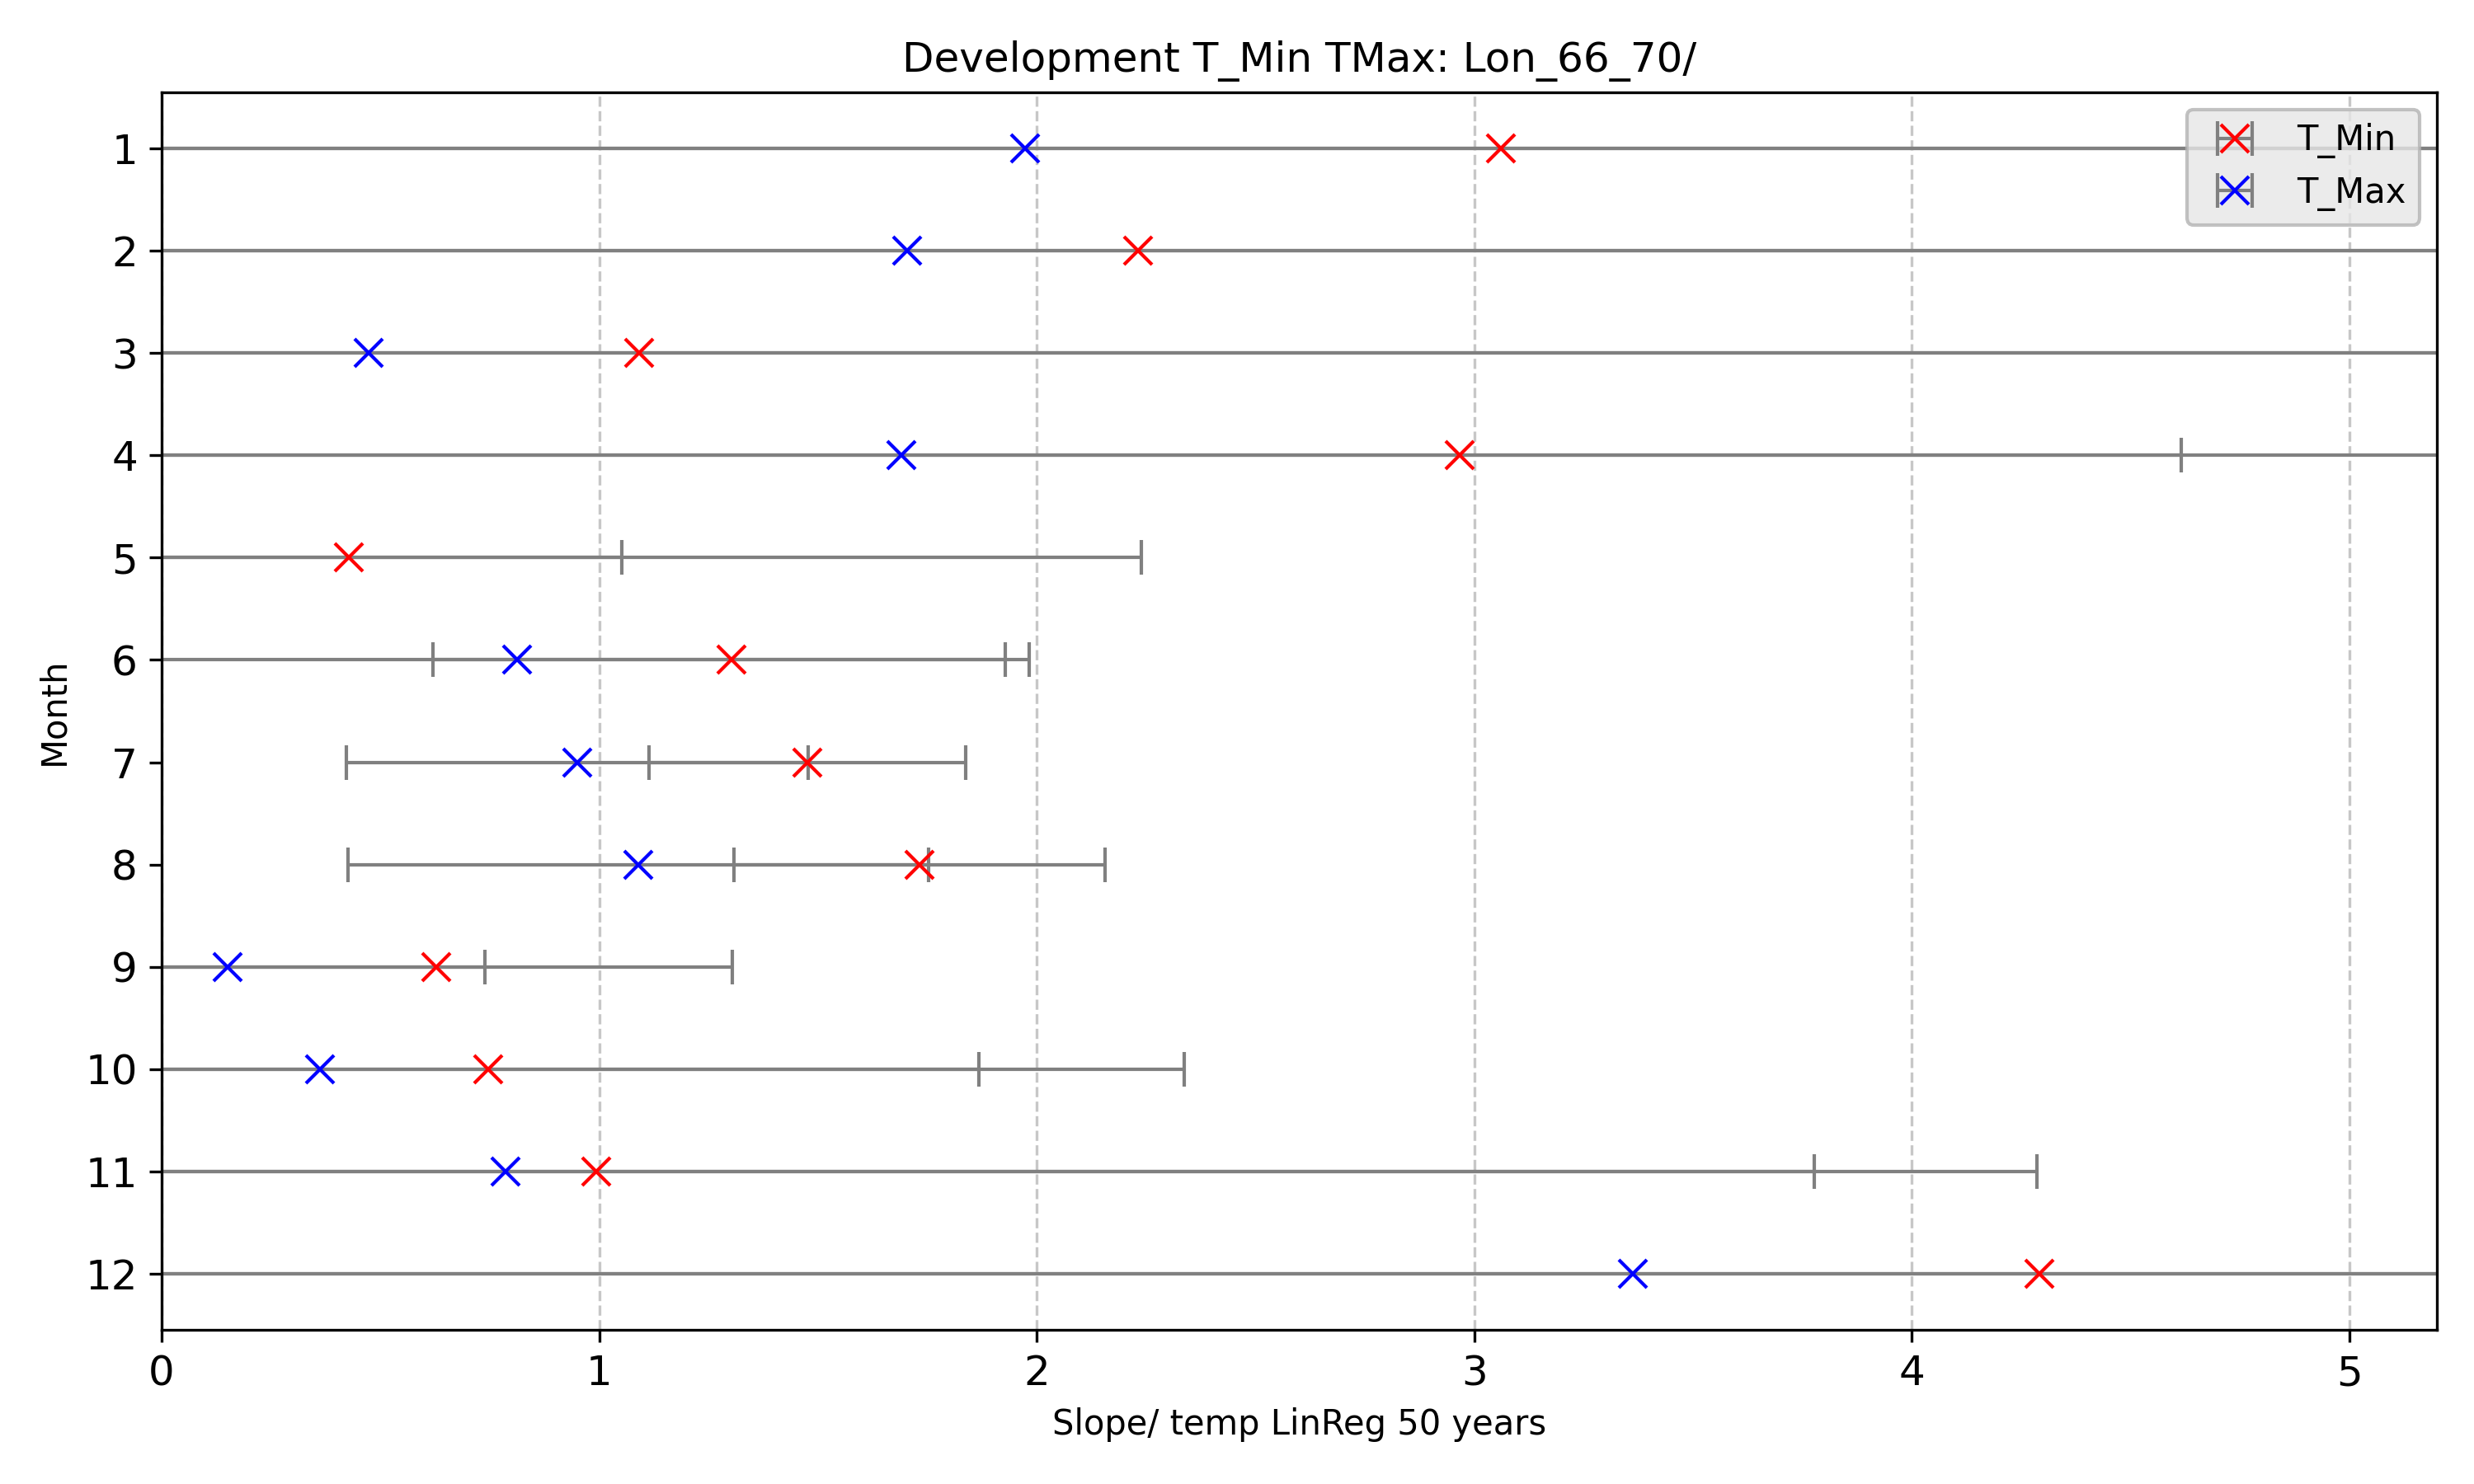
\includegraphics[width=\textwidth]{C:/Users/leonh/Desktop/Praktikum_AWI/NordPol/Lon_66_84/Fit/T_Min_T_Max.png}
        \caption{$T_{\mathrm{min/max}}$}
        \label{subfig:TMinTMax}
    \end{subfigure}

    \begin{subfigure}{0.48\textwidth}
        \centering
        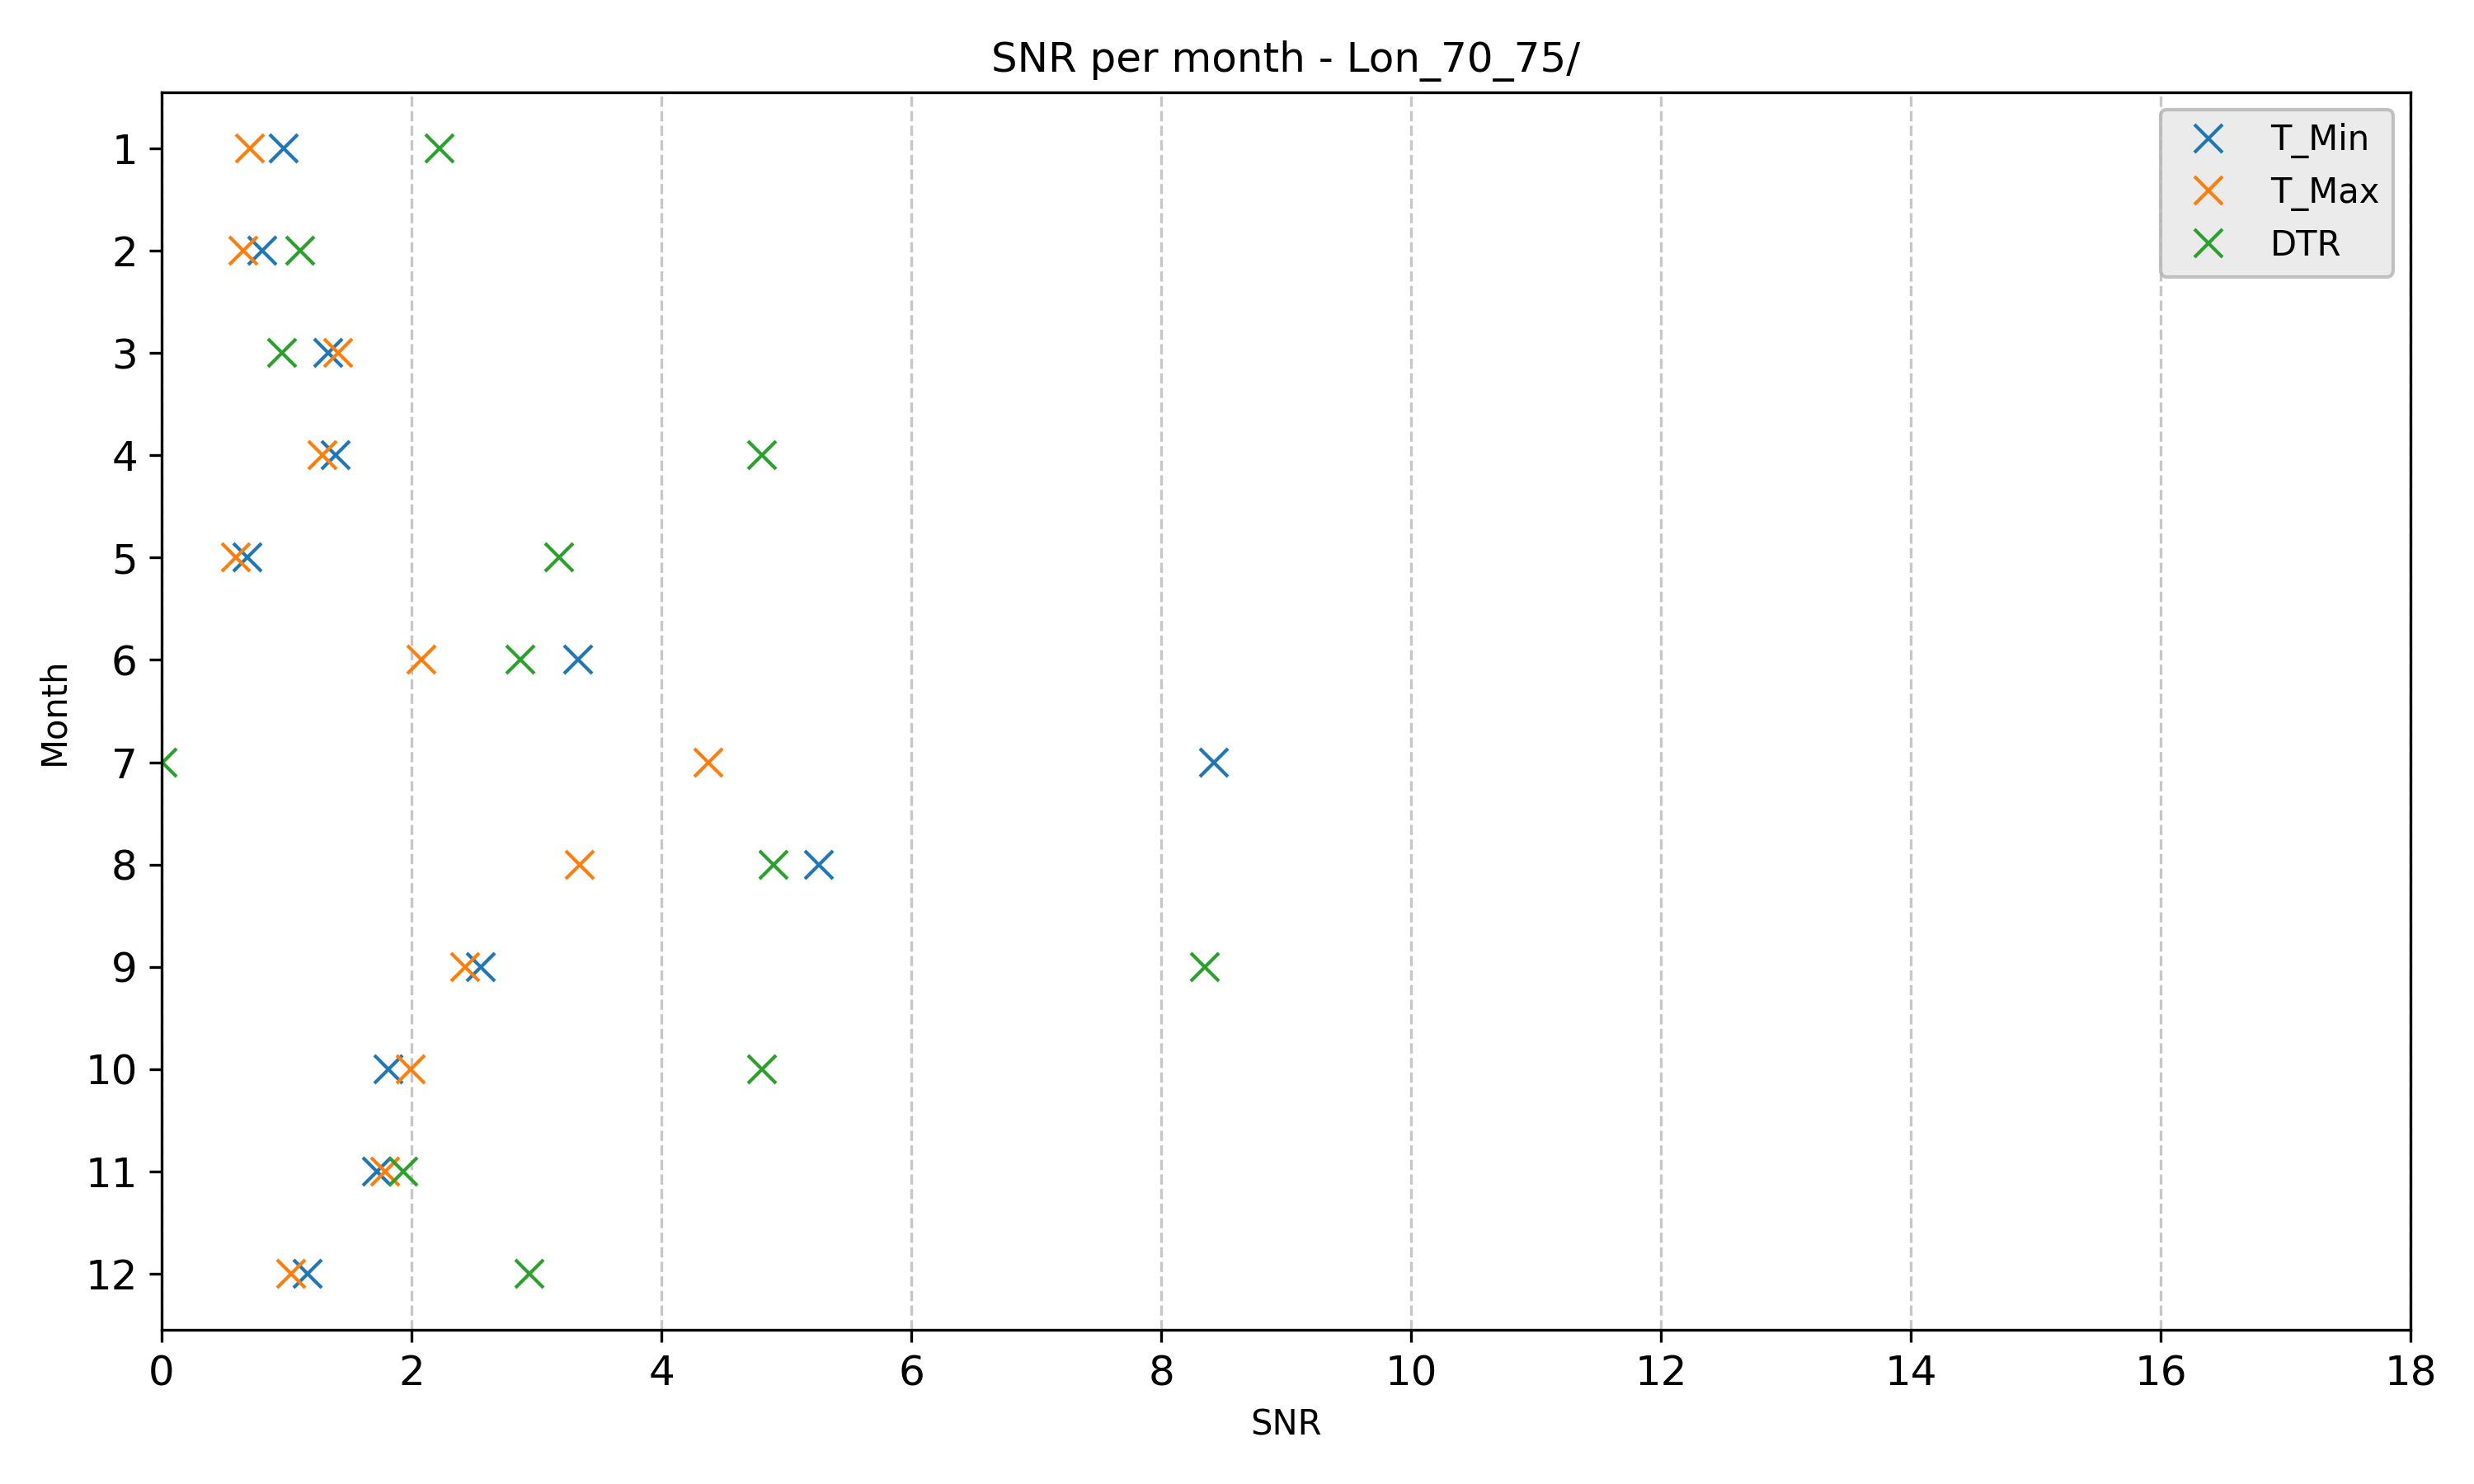
\includegraphics[width = \textwidth]{C:/Users/leonh/Desktop/Praktikum_AWI/NordPol/Lon_66_84/Fit/SNR.png}
        \caption{SNR}
        \label{subfig:SNR}
    \end{subfigure}
    \begin{subfigure}{0.43\textwidth}
        \centering
        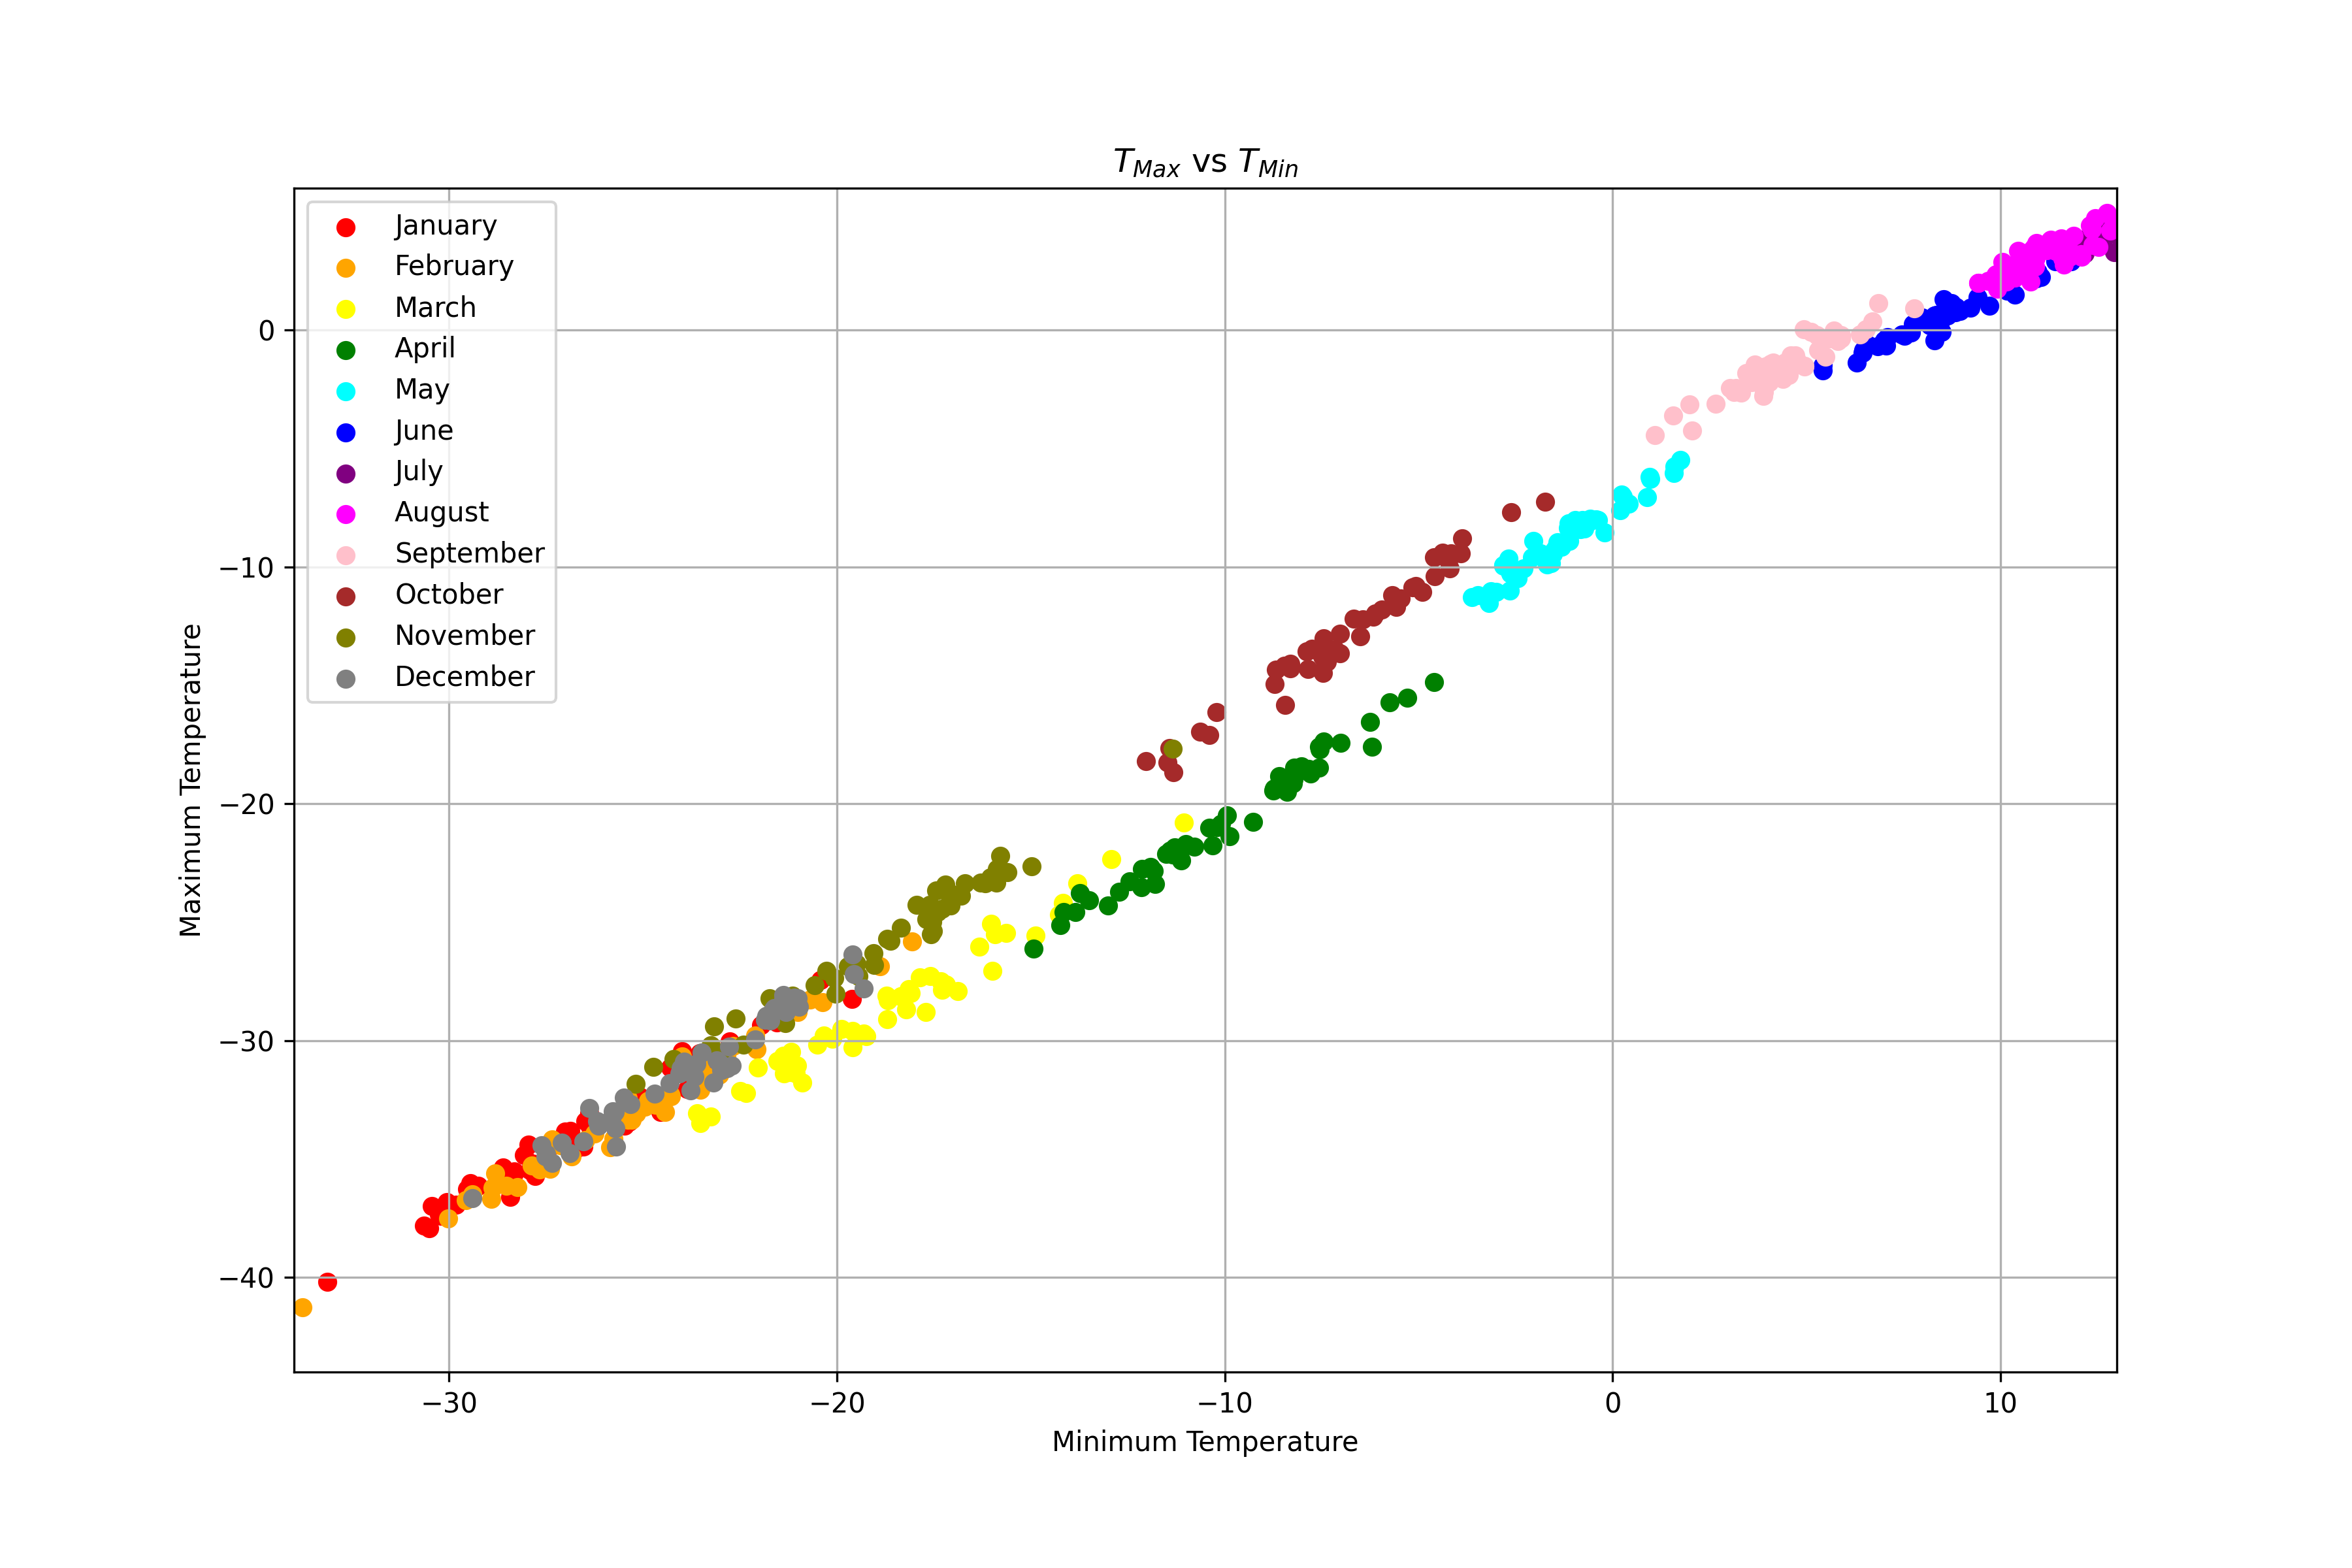
\includegraphics[width = \textwidth]{C:/Users/leonh/Desktop/Praktikum_AWI/NordPol/Lon_66_84/ScatterPlot/ScatterTMinTMax.png}
        \caption{$T_{\mathrm{min}}$ vs $T_{\mathrm{max}}$}
        \label{subfig:ScatterMinMax}
    \end{subfigure}

    \caption{Diurnal temperature range change \textbf{(a)} over 50 years for the entire polar region (66-90°). \textbf{(b)} shows, for comparison, the maximum and minimum temperature trends. The variance for these temperatures is much larger compared to \textbf{(a)}. \textbf{(c)} presents the signal-to-noise ratio for the two previous plots.}
    \label{fig:DRTentireSlopes}
\end{figure}

After taking the over all average of the weighted data\footnote{The data are weighted by area. This leads to a stronger emphasis on the "lower" latitudes. The effect of the weighting is decreasingly small at the intervals of 5° chosen later on.},
we investigate the temporal development of DTR monthly average using linear regression. To examine the significance of the trend,
the empirical variance in relation to the fit is calculated. 




As show in \cref{fig:DRTentireSlopes}, the changes in DTR are significant. But this is also true for the changes in the minimum temperature $T_{\mathrm{min}}$ as for the maximum temperature $T_{\mathrm{max}}$.
Compared to the changes in mean min./max. temperature he DRT trend does have a bigger SNR, as shown in \cref{subfig:SNR}. This can be explained through the strong correlation between maximum and 
minimum temperature (see \cref{sub@subfig:ScatterMinMax}). Due to this higher SNR, the changes in DTR could be an advantageous indicator for climatic changes in regions with high 
climate variability. Therefore, the robustness of this parameter and trends are investigated in \cref{sec:robustness}.

